% Requires: \usepackage{booktabs,longtable,tikz}
\section{Sequential-Score StateRAG Case Study}
All conditions use the same role-relative service state from match 24, set 3, rally 1. Each condition starts at 0--0 and runs 32 rallies; the winner scores one point and serves next.

\begin{table*}[t]
\centering
\caption{Sequential-score outcomes and rally lengths.}
\begin{tabular}{lrrrr}
\toprule
Condition & Target score & Opponent score & Target win (\%) & Mean length \\
\midrule
No instruction & 17 & 15 & 53.1 & 20.84 \\
Extended defensive reset with deep placement & 5 & 27 & 15.6 & 16.09 \\
Aggressive front-court net play & 30 & 2 & 93.8 & 21.38 \\
Deep back-court drive with aggressive net pressure & 4 & 28 & 12.5 & 16.09 \\
\bottomrule
\end{tabular}
\end{table*}

\subsection*{Score progression: No instruction}
\begin{center}
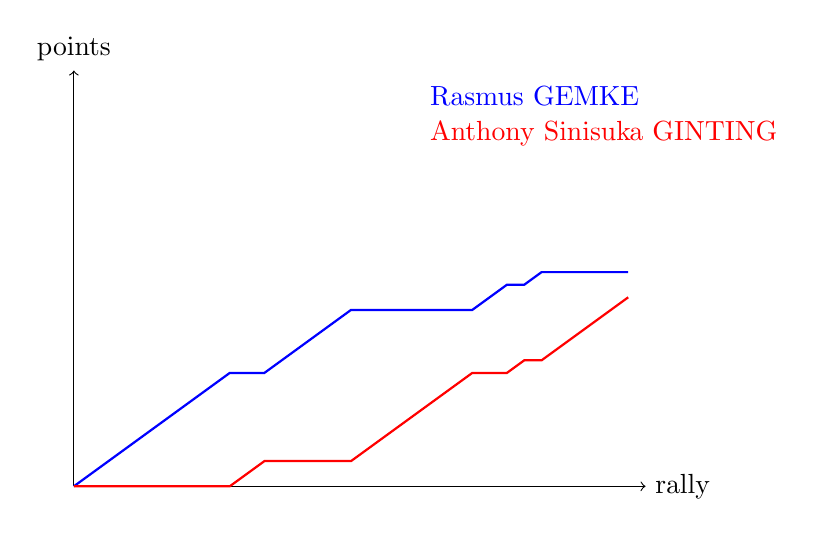
\begin{tikzpicture}[x=0.22cm,y=0.16cm]
\draw[->] (0,0) -- (33,0) node[right] {rally};
\draw[->] (0,0) -- (0,33) node[above] {points};
\draw[blue,thick] (0,0) -- (1,1) -- (2,2) -- (3,3) -- (4,4) -- (5,5) -- (6,6) -- (7,7) -- (8,8) -- (9,9) -- (10,9) -- (11,9) -- (12,10) -- (13,11) -- (14,12) -- (15,13) -- (16,14) -- (17,14) -- (18,14) -- (19,14) -- (20,14) -- (21,14) -- (22,14) -- (23,14) -- (24,15) -- (25,16) -- (26,16) -- (27,17) -- (28,17) -- (29,17) -- (30,17) -- (31,17) -- (32,17);
\draw[red,thick] (0,0) -- (1,0) -- (2,0) -- (3,0) -- (4,0) -- (5,0) -- (6,0) -- (7,0) -- (8,0) -- (9,0) -- (10,1) -- (11,2) -- (12,2) -- (13,2) -- (14,2) -- (15,2) -- (16,2) -- (17,3) -- (18,4) -- (19,5) -- (20,6) -- (21,7) -- (22,8) -- (23,9) -- (24,9) -- (25,9) -- (26,10) -- (27,10) -- (28,11) -- (29,12) -- (30,13) -- (31,14) -- (32,15);
\node[blue,anchor=west] at (20,31) {Rasmus GEMKE};
\node[red,anchor=west] at (20,28) {Anthony Sinisuka GINTING};
\end{tikzpicture}
\end{center}

\subsection*{No instruction}
\textbf{Instruction:} None\\
Representative rollout: 1; selection distance: 0.000; winner: Rasmus GEMKE.

\begin{center}
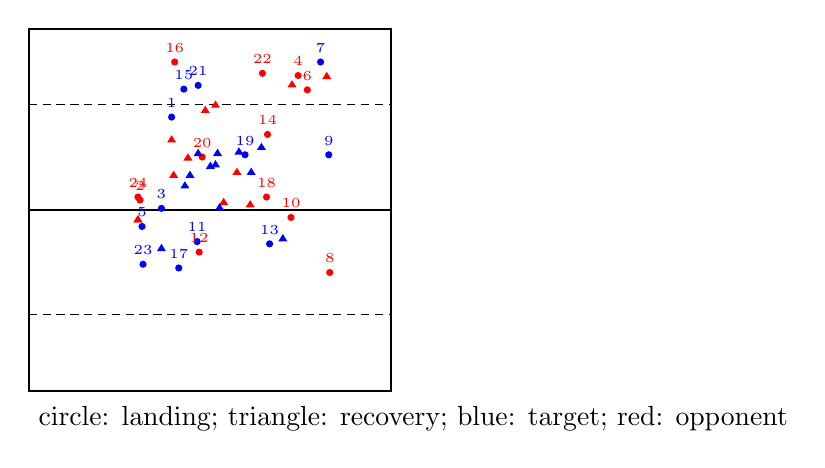
\begin{tikzpicture}[x=2.3cm,y=2.3cm]
\draw[thick] (-1,-1) rectangle (1,1);
\draw[thick] (-1,0) -- (1,0);
\draw[densely dashed] (-1,-0.58) -- (1,-0.58);
\draw[densely dashed] (-1,0.58) -- (1,0.58);
\node[anchor=west] at (-1,-1.15) {circle: landing; triangle: recovery; blue: target; red: opponent};
\fill[blue] (-0.2113,0.5125) circle (1.3pt) node[above,font=\tiny] {1};
\fill[blue] (0.0310,0.2750) -- ++(-0.025,-0.04) -- ++(0.05,0) -- cycle;
\fill[red] (-0.3859,0.0542) circle (1.3pt) node[above,font=\tiny] {2};
\fill[red] (-0.1211,0.3125) -- ++(-0.025,-0.04) -- ++(0.05,0) -- cycle;
\fill[blue] (-0.2676,0.0083) circle (1.3pt) node[above,font=\tiny] {3};
\fill[blue] (-0.2676,-0.1875) -- ++(-0.025,-0.04) -- ++(0.05,0) -- cycle;
\fill[red] (0.4873,0.7417) circle (1.3pt) node[above,font=\tiny] {4};
\fill[red] (-0.2113,0.4125) -- ++(-0.025,-0.04) -- ++(0.05,0) -- cycle;
\fill[blue] (-0.3746,-0.0917) circle (1.3pt) node[above,font=\tiny] {5};
\fill[blue] (0.2845,0.3708) -- ++(-0.025,-0.04) -- ++(0.05,0) -- cycle;
\fill[red] (0.5380,0.6625) circle (1.3pt) node[above,font=\tiny] {6};
\fill[red] (-0.2000,0.2167) -- ++(-0.025,-0.04) -- ++(0.05,0) -- cycle;
\fill[blue] (0.6113,0.8167) circle (1.3pt) node[above,font=\tiny] {7};
\fill[blue] (0.1606,0.3458) -- ++(-0.025,-0.04) -- ++(0.05,0) -- cycle;
\fill[red] (0.6620,-0.3458) circle (1.3pt) node[above,font=\tiny] {8};
\fill[red] (0.6451,0.7625) -- ++(-0.025,-0.04) -- ++(0.05,0) -- cycle;
\fill[blue] (0.6563,0.3042) circle (1.3pt) node[above,font=\tiny] {9};
\fill[blue] (0.4028,-0.1333) -- ++(-0.025,-0.04) -- ++(0.05,0) -- cycle;
\fill[red] (0.4479,-0.0417) circle (1.3pt) node[above,font=\tiny] {10};
\fill[red] (0.4535,0.7167) -- ++(-0.025,-0.04) -- ++(0.05,0) -- cycle;
\fill[blue] (-0.0704,-0.1750) circle (1.3pt) node[above,font=\tiny] {11};
\fill[blue] (-0.1099,0.2167) -- ++(-0.025,-0.04) -- ++(0.05,0) -- cycle;
\fill[red] (-0.0592,-0.2333) circle (1.3pt) node[above,font=\tiny] {12};
\fill[red] (0.0761,0.0667) -- ++(-0.025,-0.04) -- ++(0.05,0) -- cycle;
\fill[blue] (0.3296,-0.1875) circle (1.3pt) node[above,font=\tiny] {13};
\fill[blue] (0.0535,0.0375) -- ++(-0.025,-0.04) -- ++(0.05,0) -- cycle;
\fill[red] (0.3183,0.4167) circle (1.3pt) node[above,font=\tiny] {14};
\fill[red] (0.2225,0.0542) -- ++(-0.025,-0.04) -- ++(0.05,0) -- cycle;
\fill[blue] (-0.1437,0.6667) circle (1.3pt) node[above,font=\tiny] {15};
\fill[blue] (0.2282,0.2333) -- ++(-0.025,-0.04) -- ++(0.05,0) -- cycle;
\fill[red] (-0.1944,0.8167) circle (1.3pt) node[above,font=\tiny] {16};
\fill[red] (0.0310,0.6042) -- ++(-0.025,-0.04) -- ++(0.05,0) -- cycle;
\fill[blue] (-0.1718,-0.3208) circle (1.3pt) node[above,font=\tiny] {17};
\fill[blue] (0.0028,0.2667) -- ++(-0.025,-0.04) -- ++(0.05,0) -- cycle;
\fill[red] (0.3127,0.0708) circle (1.3pt) node[above,font=\tiny] {18};
\fill[red] (-0.3972,-0.0292) -- ++(-0.025,-0.04) -- ++(0.05,0) -- cycle;
\fill[blue] (0.1944,0.3042) circle (1.3pt) node[above,font=\tiny] {19};
\fill[blue] (-0.1380,0.1583) -- ++(-0.025,-0.04) -- ++(0.05,0) -- cycle;
\fill[red] (-0.0423,0.2917) circle (1.3pt) node[above,font=\tiny] {20};
\fill[red] (0.1493,0.2333) -- ++(-0.025,-0.04) -- ++(0.05,0) -- cycle;
\fill[blue] (-0.0648,0.6875) circle (1.3pt) node[above,font=\tiny] {21};
\fill[blue] (-0.0648,0.3375) -- ++(-0.025,-0.04) -- ++(0.05,0) -- cycle;
\fill[red] (0.2901,0.7542) circle (1.3pt) node[above,font=\tiny] {22};
\fill[red] (-0.0254,0.5750) -- ++(-0.025,-0.04) -- ++(0.05,0) -- cycle;
\fill[blue] (-0.3690,-0.3000) circle (1.3pt) node[above,font=\tiny] {23};
\fill[blue] (0.0423,0.3375) -- ++(-0.025,-0.04) -- ++(0.05,0) -- cycle;
\fill[red] (-0.3972,0.0708) circle (1.3pt) node[above,font=\tiny] {24};
\fill[red] (-0.3972,-0.0292) -- ++(-0.025,-0.04) -- ++(0.05,0) -- cycle;
\end{tikzpicture}
\end{center}
\begin{longtable}{rlllp{2.1cm}}
\toprule
Round & Actor & Shot & Landing area & Landing $(x,y)$ \\
\midrule
\endfirsthead
\toprule
Round & Actor & Shot & Landing area & Landing $(x,y)$ \\
\midrule
\endhead
1 & Target & Serve short & Mid Center & (-0.21, 0.51) \\
2 & Opponent & Push Shot & Rear Center & (-0.39, 0.05) \\
3 & Target & Smash & Rear Center & (-0.27, 0.01) \\
4 & Opponent & Smash Defence & Front Right Side & (0.49, 0.74) \\
5 & Target & Push Shot & Rear Center & (-0.37, -0.09) \\
6 & Opponent & Drop & Front Right Side & (0.54, 0.66) \\
7 & Target & Net Shot & Front Right Side & (0.61, 0.82) \\
8 & Opponent & Lob & Rear Right Side & (0.66, -0.35) \\
9 & Target & Drop & Mid Right Side & (0.66, 0.30) \\
10 & Opponent & Push Shot & Rear Right Side & (0.45, -0.04) \\
11 & Target & Clear & Rear Center & (-0.07, -0.18) \\
12 & Opponent & Clear & Rear Center & (-0.06, -0.23) \\
13 & Target & Clear & Rear Center & (0.33, -0.19) \\
14 & Opponent & Drop & Mid Center & (0.32, 0.42) \\
15 & Target & Net Shot & Front Center & (-0.14, 0.67) \\
16 & Opponent & Net Shot & Front Center & (-0.19, 0.82) \\
17 & Target & Lob & Rear Center & (-0.17, -0.32) \\
18 & Opponent & Smash & Rear Center & (0.31, 0.07) \\
19 & Target & Smash Defence & Mid Center & (0.19, 0.30) \\
20 & Opponent & Smash Defence & Mid Center & (-0.04, 0.29) \\
21 & Target & Net Shot & Front Center & (-0.06, 0.69) \\
22 & Opponent & Net Shot & Front Center & (0.29, 0.75) \\
23 & Target & Lob & Rear Center & (-0.37, -0.30) \\
24 & Opponent & Smash & Rear Center & (-0.40, 0.07) \\
\bottomrule
\end{longtable}

\subsection*{Score progression: Extended defensive reset with deep placement}
\begin{center}
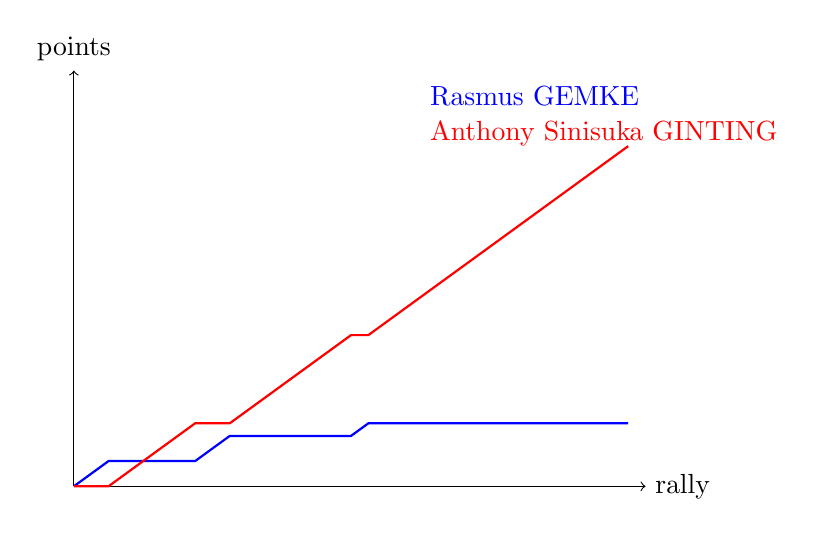
\begin{tikzpicture}[x=0.22cm,y=0.16cm]
\draw[->] (0,0) -- (33,0) node[right] {rally};
\draw[->] (0,0) -- (0,33) node[above] {points};
\draw[blue,thick] (0,0) -- (1,1) -- (2,2) -- (3,2) -- (4,2) -- (5,2) -- (6,2) -- (7,2) -- (8,3) -- (9,4) -- (10,4) -- (11,4) -- (12,4) -- (13,4) -- (14,4) -- (15,4) -- (16,4) -- (17,5) -- (18,5) -- (19,5) -- (20,5) -- (21,5) -- (22,5) -- (23,5) -- (24,5) -- (25,5) -- (26,5) -- (27,5) -- (28,5) -- (29,5) -- (30,5) -- (31,5) -- (32,5);
\draw[red,thick] (0,0) -- (1,0) -- (2,0) -- (3,1) -- (4,2) -- (5,3) -- (6,4) -- (7,5) -- (8,5) -- (9,5) -- (10,6) -- (11,7) -- (12,8) -- (13,9) -- (14,10) -- (15,11) -- (16,12) -- (17,12) -- (18,13) -- (19,14) -- (20,15) -- (21,16) -- (22,17) -- (23,18) -- (24,19) -- (25,20) -- (26,21) -- (27,22) -- (28,23) -- (29,24) -- (30,25) -- (31,26) -- (32,27);
\node[blue,anchor=west] at (20,31) {Rasmus GEMKE};
\node[red,anchor=west] at (20,28) {Anthony Sinisuka GINTING};
\end{tikzpicture}
\end{center}

\subsection*{Extended defensive reset with deep placement}
\textbf{Instruction:} Extended defensive reset with deep placement. Focus on deep defensive resets to extend rallies and maintain distance from the opponent.\\
Representative rollout: 23; selection distance: 0.000; winner: Anthony Sinisuka GINTING.

\begin{center}
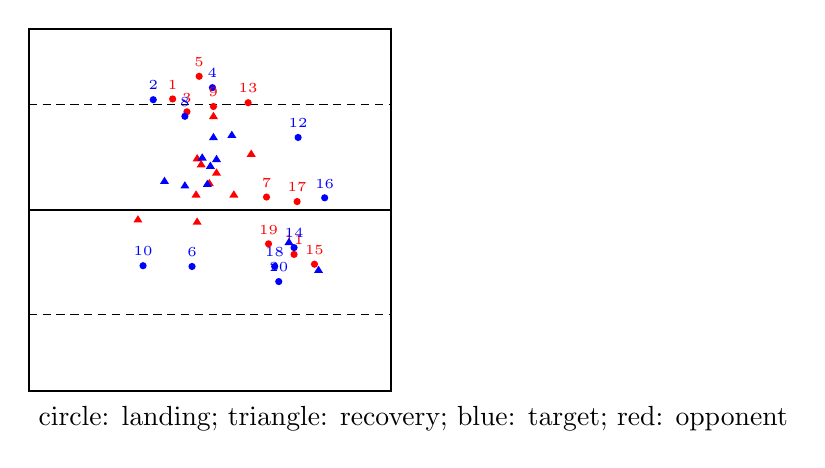
\begin{tikzpicture}[x=2.3cm,y=2.3cm]
\draw[thick] (-1,-1) rectangle (1,1);
\draw[thick] (-1,0) -- (1,0);
\draw[densely dashed] (-1,-0.58) -- (1,-0.58);
\draw[densely dashed] (-1,0.58) -- (1,0.58);
\node[anchor=west] at (-1,-1.15) {circle: landing; triangle: recovery; blue: target; red: opponent};
\fill[red] (-0.2056,0.6125) circle (1.3pt) node[above,font=\tiny] {1};
\fill[red] (0.0366,0.2292) -- ++(-0.025,-0.04) -- ++(0.05,0) -- cycle;
\fill[blue] (-0.3127,0.6083) circle (1.3pt) node[above,font=\tiny] {2};
\fill[blue] (0.0197,0.4250) -- ++(-0.025,-0.04) -- ++(0.05,0) -- cycle;
\fill[red] (-0.1268,0.5417) circle (1.3pt) node[above,font=\tiny] {3};
\fill[red] (-0.0704,0.3083) -- ++(-0.025,-0.04) -- ++(0.05,0) -- cycle;
\fill[blue] (0.0141,0.6750) circle (1.3pt) node[above,font=\tiny] {4};
\fill[blue] (0.1211,0.4375) -- ++(-0.025,-0.04) -- ++(0.05,0) -- cycle;
\fill[red] (-0.0592,0.7375) circle (1.3pt) node[above,font=\tiny] {5};
\fill[red] (0.0197,0.5417) -- ++(-0.025,-0.04) -- ++(0.05,0) -- cycle;
\fill[blue] (-0.0986,-0.3125) circle (1.3pt) node[above,font=\tiny] {6};
\fill[blue] (0.0028,0.2667) -- ++(-0.025,-0.04) -- ++(0.05,0) -- cycle;
\fill[red] (0.3127,0.0708) circle (1.3pt) node[above,font=\tiny] {7};
\fill[red] (-0.3972,-0.0292) -- ++(-0.025,-0.04) -- ++(0.05,0) -- cycle;
\fill[blue] (-0.1380,0.5167) circle (1.3pt) node[above,font=\tiny] {8};
\fill[blue] (-0.1380,0.1583) -- ++(-0.025,-0.04) -- ++(0.05,0) -- cycle;
\fill[red] (0.0197,0.5708) circle (1.3pt) node[above,font=\tiny] {9};
\fill[red] (-0.0479,0.2750) -- ++(-0.025,-0.04) -- ++(0.05,0) -- cycle;
\fill[blue] (-0.3690,-0.3083) circle (1.3pt) node[above,font=\tiny] {10};
\fill[blue] (0.0366,0.3042) -- ++(-0.025,-0.04) -- ++(0.05,0) -- cycle;
\fill[red] (0.4648,-0.2458) circle (1.3pt) node[above,font=\tiny] {11};
\fill[red] (-0.0761,0.1083) -- ++(-0.025,-0.04) -- ++(0.05,0) -- cycle;
\fill[blue] (0.4873,0.4000) circle (1.3pt) node[above,font=\tiny] {12};
\fill[blue] (0.4366,-0.1542) -- ++(-0.025,-0.04) -- ++(0.05,0) -- cycle;
\fill[red] (0.2113,0.5917) circle (1.3pt) node[above,font=\tiny] {13};
\fill[red] (0.2282,0.3333) -- ++(-0.025,-0.04) -- ++(0.05,0) -- cycle;
\fill[blue] (0.4648,-0.2083) circle (1.3pt) node[above,font=\tiny] {14};
\fill[blue] (-0.0423,0.3125) -- ++(-0.025,-0.04) -- ++(0.05,0) -- cycle;
\fill[red] (0.5775,-0.3000) circle (1.3pt) node[above,font=\tiny] {15};
\fill[red] (-0.0028,0.1708) -- ++(-0.025,-0.04) -- ++(0.05,0) -- cycle;
\fill[blue] (0.6338,0.0667) circle (1.3pt) node[above,font=\tiny] {16};
\fill[blue] (0.6000,-0.3083) -- ++(-0.025,-0.04) -- ++(0.05,0) -- cycle;
\fill[red] (0.4817,0.0458) circle (1.3pt) node[above,font=\tiny] {17};
\fill[red] (0.1324,0.1083) -- ++(-0.025,-0.04) -- ++(0.05,0) -- cycle;
\fill[blue] (0.3577,-0.3125) circle (1.3pt) node[above,font=\tiny] {18};
\fill[blue] (-0.2507,0.1833) -- ++(-0.025,-0.04) -- ++(0.05,0) -- cycle;
\fill[red] (0.3239,-0.1875) circle (1.3pt) node[above,font=\tiny] {19};
\fill[red] (-0.0704,-0.0417) -- ++(-0.025,-0.04) -- ++(0.05,0) -- cycle;
\fill[blue] (0.3803,-0.3958) circle (1.3pt) node[above,font=\tiny] {20};
\fill[blue] (-0.0141,0.1667) -- ++(-0.025,-0.04) -- ++(0.05,0) -- cycle;
\end{tikzpicture}
\end{center}
\begin{longtable}{rlllp{2.1cm}}
\toprule
Round & Actor & Shot & Landing area & Landing $(x,y)$ \\
\midrule
\endfirsthead
\toprule
Round & Actor & Shot & Landing area & Landing $(x,y)$ \\
\midrule
\endhead
1 & Opponent & Serve short & Front Center & (-0.21, 0.61) \\
2 & Target & Net Shot & Front Center & (-0.31, 0.61) \\
3 & Opponent & Net Shot & Front Center & (-0.13, 0.54) \\
4 & Target & Net Shot & Front Center & (0.01, 0.68) \\
5 & Opponent & Net Shot & Front Center & (-0.06, 0.74) \\
6 & Target & Lob & Rear Center & (-0.10, -0.31) \\
7 & Opponent & Smash & Rear Center & (0.31, 0.07) \\
8 & Target & Smash Defence & Mid Center & (-0.14, 0.52) \\
9 & Opponent & Net Shot & Front Center & (0.02, 0.57) \\
10 & Target & Lob & Rear Center & (-0.37, -0.31) \\
11 & Opponent & Clear & Rear Right Side & (0.46, -0.25) \\
12 & Target & Drop & Mid Right Side & (0.49, 0.40) \\
13 & Opponent & Net Shot & Front Center & (0.21, 0.59) \\
14 & Target & Lob & Rear Right Side & (0.46, -0.21) \\
15 & Opponent & Clear & Rear Right Side & (0.58, -0.30) \\
16 & Target & Smash & Rear Right Side & (0.63, 0.07) \\
17 & Opponent & Smash Defence & Rear Right Side & (0.48, 0.05) \\
18 & Target & Lob & Rear Center & (0.36, -0.31) \\
19 & Opponent & Clear & Rear Center & (0.32, -0.19) \\
20 & Target & Clear & Deep Right Corner & (0.38, -0.40) \\
\bottomrule
\end{longtable}

\subsection*{Score progression: Aggressive front-court net play}
\begin{center}
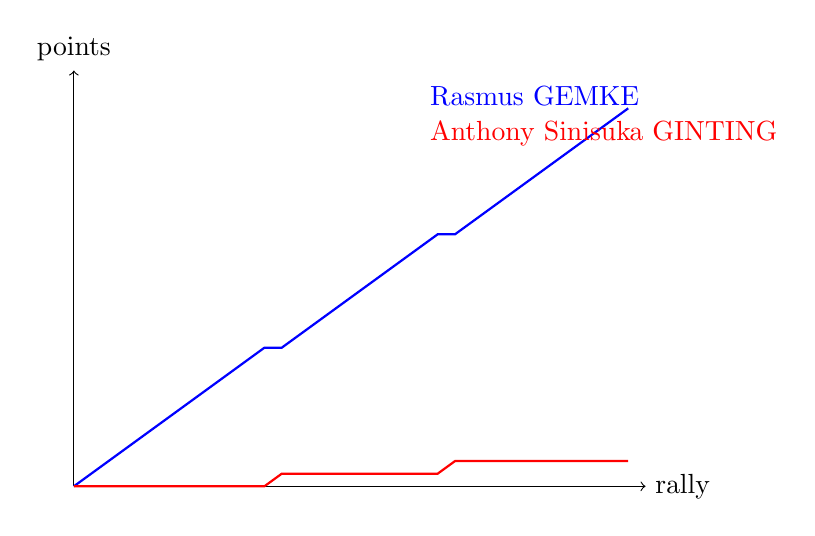
\begin{tikzpicture}[x=0.22cm,y=0.16cm]
\draw[->] (0,0) -- (33,0) node[right] {rally};
\draw[->] (0,0) -- (0,33) node[above] {points};
\draw[blue,thick] (0,0) -- (1,1) -- (2,2) -- (3,3) -- (4,4) -- (5,5) -- (6,6) -- (7,7) -- (8,8) -- (9,9) -- (10,10) -- (11,11) -- (12,11) -- (13,12) -- (14,13) -- (15,14) -- (16,15) -- (17,16) -- (18,17) -- (19,18) -- (20,19) -- (21,20) -- (22,20) -- (23,21) -- (24,22) -- (25,23) -- (26,24) -- (27,25) -- (28,26) -- (29,27) -- (30,28) -- (31,29) -- (32,30);
\draw[red,thick] (0,0) -- (1,0) -- (2,0) -- (3,0) -- (4,0) -- (5,0) -- (6,0) -- (7,0) -- (8,0) -- (9,0) -- (10,0) -- (11,0) -- (12,1) -- (13,1) -- (14,1) -- (15,1) -- (16,1) -- (17,1) -- (18,1) -- (19,1) -- (20,1) -- (21,1) -- (22,2) -- (23,2) -- (24,2) -- (25,2) -- (26,2) -- (27,2) -- (28,2) -- (29,2) -- (30,2) -- (31,2) -- (32,2);
\node[blue,anchor=west] at (20,31) {Rasmus GEMKE};
\node[red,anchor=west] at (20,28) {Anthony Sinisuka GINTING};
\end{tikzpicture}
\end{center}

\subsection*{Aggressive front-court net play}
\textbf{Instruction:} Aggressive front-court net play. Focus all shots on the front court to force the opponent to the net and keep rallies short.\\
Representative rollout: 1; selection distance: 0.000; winner: Rasmus GEMKE.

\begin{center}
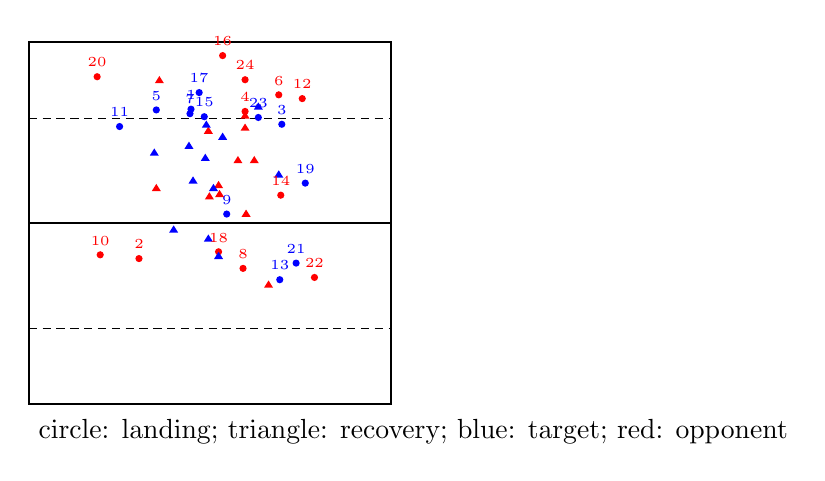
\begin{tikzpicture}[x=2.3cm,y=2.3cm]
\draw[thick] (-1,-1) rectangle (1,1);
\draw[thick] (-1,0) -- (1,0);
\draw[densely dashed] (-1,-0.58) -- (1,-0.58);
\draw[densely dashed] (-1,0.58) -- (1,0.58);
\node[anchor=west] at (-1,-1.15) {circle: landing; triangle: recovery; blue: target; red: opponent};
\fill[blue] (-0.1042,0.6292) circle (1.3pt) node[above,font=\tiny] {1};
\fill[blue] (-0.1155,0.4500) -- ++(-0.025,-0.04) -- ++(0.05,0) -- cycle;
\fill[red] (-0.3915,-0.1958) circle (1.3pt) node[above,font=\tiny] {2};
\fill[red] (0.0479,0.2333) -- ++(-0.025,-0.04) -- ++(0.05,0) -- cycle;
\fill[blue] (0.3972,0.5458) circle (1.3pt) node[above,font=\tiny] {3};
\fill[blue] (-0.2000,-0.0125) -- ++(-0.025,-0.04) -- ++(0.05,0) -- cycle;
\fill[red] (0.1944,0.6167) circle (1.3pt) node[above,font=\tiny] {4};
\fill[red] (0.1944,0.6167) -- ++(-0.025,-0.04) -- ++(0.05,0) -- cycle;
\fill[blue] (-0.2958,0.6250) circle (1.3pt) node[above,font=\tiny] {5};
\fill[blue] (0.0704,0.5000) -- ++(-0.025,-0.04) -- ++(0.05,0) -- cycle;
\fill[red] (0.3803,0.7083) circle (1.3pt) node[above,font=\tiny] {6};
\fill[red] (-0.2789,0.8125) -- ++(-0.025,-0.04) -- ++(0.05,0) -- cycle;
\fill[blue] (-0.1099,0.6042) circle (1.3pt) node[above,font=\tiny] {7};
\fill[blue] (0.0197,0.2167) -- ++(-0.025,-0.04) -- ++(0.05,0) -- cycle;
\fill[red] (0.1831,-0.2500) circle (1.3pt) node[above,font=\tiny] {8};
\fill[red] (0.1549,0.3708) -- ++(-0.025,-0.04) -- ++(0.05,0) -- cycle;
\fill[blue] (0.0930,0.0500) circle (1.3pt) node[above,font=\tiny] {9};
\fill[blue] (0.3803,0.2917) -- ++(-0.025,-0.04) -- ++(0.05,0) -- cycle;
\fill[red] (-0.6056,-0.1750) circle (1.3pt) node[above,font=\tiny] {10};
\fill[red] (0.2000,0.0750) -- ++(-0.025,-0.04) -- ++(0.05,0) -- cycle;
\fill[blue] (-0.4986,0.5333) circle (1.3pt) node[above,font=\tiny] {11};
\fill[blue] (-0.0085,-0.0625) -- ++(-0.025,-0.04) -- ++(0.05,0) -- cycle;
\fill[red] (0.5099,0.6875) circle (1.3pt) node[above,font=\tiny] {12};
\fill[red] (-0.2958,0.2167) -- ++(-0.025,-0.04) -- ++(0.05,0) -- cycle;
\fill[blue] (0.3859,-0.3125) circle (1.3pt) node[above,font=\tiny] {13};
\fill[blue] (-0.0930,0.2583) -- ++(-0.025,-0.04) -- ++(0.05,0) -- cycle;
\fill[red] (0.3915,0.1542) circle (1.3pt) node[above,font=\tiny] {14};
\fill[red] (0.3239,-0.3167) -- ++(-0.025,-0.04) -- ++(0.05,0) -- cycle;
\fill[blue] (-0.0310,0.5875) circle (1.3pt) node[above,font=\tiny] {15};
\fill[blue] (-0.0254,0.3833) -- ++(-0.025,-0.04) -- ++(0.05,0) -- cycle;
\fill[red] (0.0704,0.9250) circle (1.3pt) node[above,font=\tiny] {16};
\fill[red] (-0.0085,0.5333) -- ++(-0.025,-0.04) -- ++(0.05,0) -- cycle;
\fill[blue] (-0.0592,0.7208) circle (1.3pt) node[above,font=\tiny] {17};
\fill[blue] (-0.0197,0.5667) -- ++(-0.025,-0.04) -- ++(0.05,0) -- cycle;
\fill[red] (0.0479,-0.1583) circle (1.3pt) node[above,font=\tiny] {18};
\fill[red] (0.0535,0.1833) -- ++(-0.025,-0.04) -- ++(0.05,0) -- cycle;
\fill[blue] (0.5268,0.2208) circle (1.3pt) node[above,font=\tiny] {19};
\fill[blue] (0.0479,-0.1583) -- ++(-0.025,-0.04) -- ++(0.05,0) -- cycle;
\fill[red] (-0.6225,0.8083) circle (1.3pt) node[above,font=\tiny] {20};
\fill[red] (0.2451,0.3708) -- ++(-0.025,-0.04) -- ++(0.05,0) -- cycle;
\fill[blue] (0.4761,-0.2208) circle (1.3pt) node[above,font=\tiny] {21};
\fill[blue] (-0.3070,0.4125) -- ++(-0.025,-0.04) -- ++(0.05,0) -- cycle;
\fill[red] (0.5775,-0.3000) circle (1.3pt) node[above,font=\tiny] {22};
\fill[red] (-0.0028,0.1708) -- ++(-0.025,-0.04) -- ++(0.05,0) -- cycle;
\fill[blue] (0.2676,0.5833) circle (1.3pt) node[above,font=\tiny] {23};
\fill[blue] (0.2676,0.6667) -- ++(-0.025,-0.04) -- ++(0.05,0) -- cycle;
\fill[red] (0.1944,0.7917) circle (1.3pt) node[above,font=\tiny] {24};
\fill[red] (0.1944,0.5500) -- ++(-0.025,-0.04) -- ++(0.05,0) -- cycle;
\end{tikzpicture}
\end{center}
\begin{longtable}{rlllp{2.1cm}}
\toprule
Round & Actor & Shot & Landing area & Landing $(x,y)$ \\
\midrule
\endfirsthead
\toprule
Round & Actor & Shot & Landing area & Landing $(x,y)$ \\
\midrule
\endhead
1 & Target & Serve short & Front Center & (-0.10, 0.63) \\
2 & Opponent & Lob & Rear Center & (-0.39, -0.20) \\
3 & Target & Drop & Front Center & (0.40, 0.55) \\
4 & Opponent & Push Shot & Front Center & (0.19, 0.62) \\
5 & Target & Clear & Front Center & (-0.30, 0.62) \\
6 & Opponent & Smash & Front Center & (0.38, 0.71) \\
7 & Target & Smash Defence & Front Center & (-0.11, 0.60) \\
8 & Opponent & Push Shot & Rear Center & (0.18, -0.25) \\
9 & Target & Clear & Rear Center & (0.09, 0.05) \\
10 & Opponent & Clear & Rear Left Side & (-0.61, -0.18) \\
11 & Target & Drop & Front Left Side & (-0.50, 0.53) \\
12 & Opponent & Net Shot & Front Right Side & (0.51, 0.69) \\
13 & Target & Lob & Rear Center & (0.39, -0.31) \\
14 & Opponent & Smash & Mid Center & (0.39, 0.15) \\
15 & Target & Smash Defence & Front Center & (-0.03, 0.59) \\
16 & Opponent & Net Shot & Front Center & (0.07, 0.93) \\
17 & Target & Net Shot & Front Center & (-0.06, 0.72) \\
18 & Opponent & Lob & Rear Center & (0.05, -0.16) \\
19 & Target & Smash & Mid Right Side & (0.53, 0.22) \\
20 & Opponent & Smash Defence & Front Left Side & (-0.62, 0.81) \\
21 & Target & Lob & Rear Right Side & (0.48, -0.22) \\
22 & Opponent & Clear & Rear Right Side & (0.58, -0.30) \\
23 & Target & Smash & Front Center & (0.27, 0.58) \\
24 & Opponent & Net Shot & Front Center & (0.19, 0.79) \\
\bottomrule
\end{longtable}

\subsection*{Score progression: Deep back-court drive with aggressive net pressure}
\begin{center}
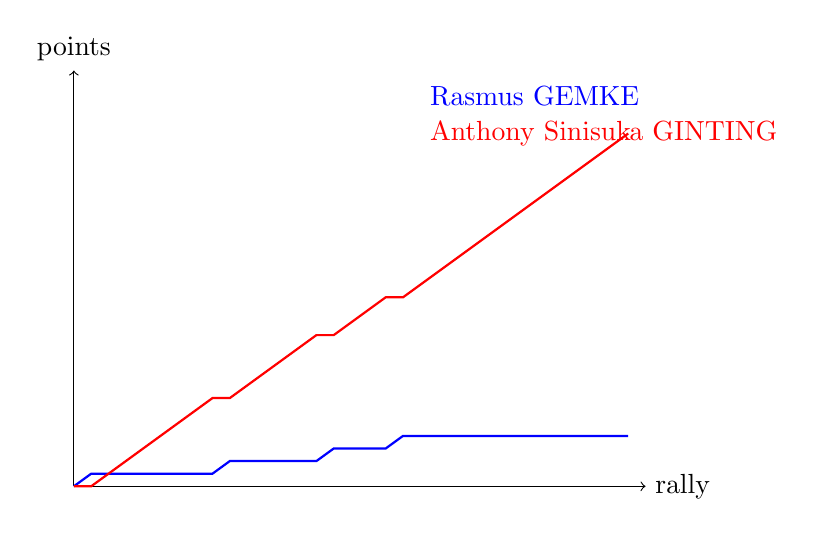
\begin{tikzpicture}[x=0.22cm,y=0.16cm]
\draw[->] (0,0) -- (33,0) node[right] {rally};
\draw[->] (0,0) -- (0,33) node[above] {points};
\draw[blue,thick] (0,0) -- (1,1) -- (2,1) -- (3,1) -- (4,1) -- (5,1) -- (6,1) -- (7,1) -- (8,1) -- (9,2) -- (10,2) -- (11,2) -- (12,2) -- (13,2) -- (14,2) -- (15,3) -- (16,3) -- (17,3) -- (18,3) -- (19,4) -- (20,4) -- (21,4) -- (22,4) -- (23,4) -- (24,4) -- (25,4) -- (26,4) -- (27,4) -- (28,4) -- (29,4) -- (30,4) -- (31,4) -- (32,4);
\draw[red,thick] (0,0) -- (1,0) -- (2,1) -- (3,2) -- (4,3) -- (5,4) -- (6,5) -- (7,6) -- (8,7) -- (9,7) -- (10,8) -- (11,9) -- (12,10) -- (13,11) -- (14,12) -- (15,12) -- (16,13) -- (17,14) -- (18,15) -- (19,15) -- (20,16) -- (21,17) -- (22,18) -- (23,19) -- (24,20) -- (25,21) -- (26,22) -- (27,23) -- (28,24) -- (29,25) -- (30,26) -- (31,27) -- (32,28);
\node[blue,anchor=west] at (20,31) {Rasmus GEMKE};
\node[red,anchor=west] at (20,28) {Anthony Sinisuka GINTING};
\end{tikzpicture}
\end{center}

\subsection*{Deep back-court drive with aggressive net pressure}
\textbf{Instruction:} Deep back-court drive with aggressive net pressure. Drive hard to the back corners to force the opponent deep, then immediately attack the net with sharp drives.\\
Representative rollout: 2; selection distance: 0.000; winner: Anthony Sinisuka GINTING.

\begin{center}
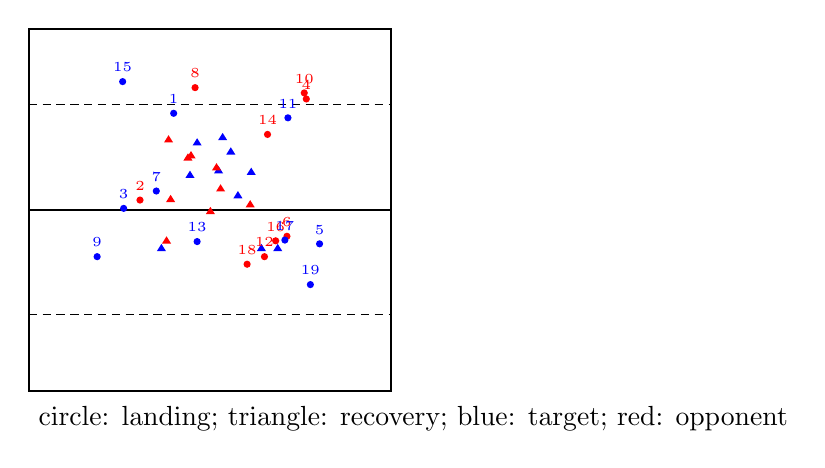
\begin{tikzpicture}[x=2.3cm,y=2.3cm]
\draw[thick] (-1,-1) rectangle (1,1);
\draw[thick] (-1,0) -- (1,0);
\draw[densely dashed] (-1,-0.58) -- (1,-0.58);
\draw[densely dashed] (-1,0.58) -- (1,0.58);
\node[anchor=west] at (-1,-1.15) {circle: landing; triangle: recovery; blue: target; red: opponent};
\fill[blue] (-0.2000,0.5333) circle (1.3pt) node[above,font=\tiny] {1};
\fill[blue] (0.0479,0.2417) -- ++(-0.025,-0.04) -- ++(0.05,0) -- cycle;
\fill[red] (-0.3859,0.0542) circle (1.3pt) node[above,font=\tiny] {2};
\fill[red] (-0.1211,0.3125) -- ++(-0.025,-0.04) -- ++(0.05,0) -- cycle;
\fill[blue] (-0.4761,0.0083) circle (1.3pt) node[above,font=\tiny] {3};
\fill[blue] (-0.2676,-0.1875) -- ++(-0.025,-0.04) -- ++(0.05,0) -- cycle;
\fill[red] (0.5324,0.6125) circle (1.3pt) node[above,font=\tiny] {4};
\fill[red] (-0.2169,0.0833) -- ++(-0.025,-0.04) -- ++(0.05,0) -- cycle;
\fill[blue] (0.6056,-0.1875) circle (1.3pt) node[above,font=\tiny] {5};
\fill[blue] (-0.0704,0.3958) -- ++(-0.025,-0.04) -- ++(0.05,0) -- cycle;
\fill[red] (0.4254,-0.1458) circle (1.3pt) node[above,font=\tiny] {6};
\fill[red] (0.0028,0.0167) -- ++(-0.025,-0.04) -- ++(0.05,0) -- cycle;
\fill[blue] (-0.2958,0.1042) circle (1.3pt) node[above,font=\tiny] {7};
\fill[blue] (0.2845,-0.1875) -- ++(-0.025,-0.04) -- ++(0.05,0) -- cycle;
\fill[red] (-0.0817,0.6750) circle (1.3pt) node[above,font=\tiny] {8};
\fill[red] (-0.1042,0.3250) -- ++(-0.025,-0.04) -- ++(0.05,0) -- cycle;
\fill[blue] (-0.6225,-0.2583) circle (1.3pt) node[above,font=\tiny] {9};
\fill[blue] (0.0704,0.4250) -- ++(-0.025,-0.04) -- ++(0.05,0) -- cycle;
\fill[red] (0.5211,0.6458) circle (1.3pt) node[above,font=\tiny] {10};
\fill[red] (-0.2394,-0.1458) -- ++(-0.025,-0.04) -- ++(0.05,0) -- cycle;
\fill[blue] (0.4310,0.5083) circle (1.3pt) node[above,font=\tiny] {11};
\fill[blue] (0.1155,0.3458) -- ++(-0.025,-0.04) -- ++(0.05,0) -- cycle;
\fill[red] (0.3014,-0.2583) circle (1.3pt) node[above,font=\tiny] {12};
\fill[red] (0.0366,0.2583) -- ++(-0.025,-0.04) -- ++(0.05,0) -- cycle;
\fill[blue] (-0.0704,-0.1750) circle (1.3pt) node[above,font=\tiny] {13};
\fill[blue] (-0.1099,0.2167) -- ++(-0.025,-0.04) -- ++(0.05,0) -- cycle;
\fill[red] (0.3183,0.4167) circle (1.3pt) node[above,font=\tiny] {14};
\fill[red] (0.2225,0.0542) -- ++(-0.025,-0.04) -- ++(0.05,0) -- cycle;
\fill[blue] (-0.4817,0.7083) circle (1.3pt) node[above,font=\tiny] {15};
\fill[blue] (0.2282,0.2333) -- ++(-0.025,-0.04) -- ++(0.05,0) -- cycle;
\fill[red] (0.3634,-0.1708) circle (1.3pt) node[above,font=\tiny] {16};
\fill[red] (-0.2282,0.4125) -- ++(-0.025,-0.04) -- ++(0.05,0) -- cycle;
\fill[blue] (0.4141,-0.1667) circle (1.3pt) node[above,font=\tiny] {17};
\fill[blue] (0.1549,0.1042) -- ++(-0.025,-0.04) -- ++(0.05,0) -- cycle;
\fill[red] (0.2056,-0.3000) circle (1.3pt) node[above,font=\tiny] {18};
\fill[red] (0.0592,0.1417) -- ++(-0.025,-0.04) -- ++(0.05,0) -- cycle;
\fill[blue] (0.5549,-0.4125) circle (1.3pt) node[above,font=\tiny] {19};
\fill[blue] (0.3746,-0.1875) -- ++(-0.025,-0.04) -- ++(0.05,0) -- cycle;
\end{tikzpicture}
\end{center}
\begin{longtable}{rlllp{2.1cm}}
\toprule
Round & Actor & Shot & Landing area & Landing $(x,y)$ \\
\midrule
\endfirsthead
\toprule
Round & Actor & Shot & Landing area & Landing $(x,y)$ \\
\midrule
\endhead
1 & Target & Serve short & Front Center & (-0.20, 0.53) \\
2 & Opponent & Push Shot & Rear Center & (-0.39, 0.05) \\
3 & Target & Smash & Rear Left Side & (-0.48, 0.01) \\
4 & Opponent & Smash Defence & Front Right Side & (0.53, 0.61) \\
5 & Target & Push Shot & Rear Right Side & (0.61, -0.19) \\
6 & Opponent & Clear & Rear Right Side & (0.43, -0.15) \\
7 & Target & Smash & Mid Center & (-0.30, 0.10) \\
8 & Opponent & Smash Defence & Front Center & (-0.08, 0.68) \\
9 & Target & Push Shot & Rear Left Side & (-0.62, -0.26) \\
10 & Opponent & Drop & Front Right Side & (0.52, 0.65) \\
11 & Target & Net Shot & Mid Right Side & (0.43, 0.51) \\
12 & Opponent & Push Shot & Rear Center & (0.30, -0.26) \\
13 & Target & Clear & Rear Center & (-0.07, -0.18) \\
14 & Opponent & Drop & Mid Center & (0.32, 0.42) \\
15 & Target & Net Shot & Front Left Side & (-0.48, 0.71) \\
16 & Opponent & Lob & Rear Center & (0.36, -0.17) \\
17 & Target & Clear & Rear Right Side & (0.41, -0.17) \\
18 & Opponent & Clear & Rear Center & (0.21, -0.30) \\
19 & Target & Clear & Deep Right Corner & (0.55, -0.41) \\
\bottomrule
\end{longtable}

